\chapter{Implementation of an IoT based Electronic Voting Machine}

\section{Hardware Reference}

\begin{table}[h!]
    \centering
    \begin{tabular}{|l|c|p{5cm}|}
        \hline
        \textbf{Basic Component List} & \textbf{Number} & \textbf{Notes} \\
        \hline
        NodeMCU ESP32  & 1 & Development board for prototyping \\
        \hline
        1,8" LCD Display Module  & 1 & 128x160 Pixel, includes microSD Slot \\
        \hline
        Button module with 2 Buttons & 1 & For interacting \\
        \hline
		Jumper Wires Female to Male & 22 & For connecting components \\
        \hline
        Breadboard & 1 & For building circuits \\
        \hline
    \end{tabular}
    \caption{Basic Component List for Guardian Prototype}\label{tab:basic-component-list}
\end{table}

\begin{figure}
	\centering
	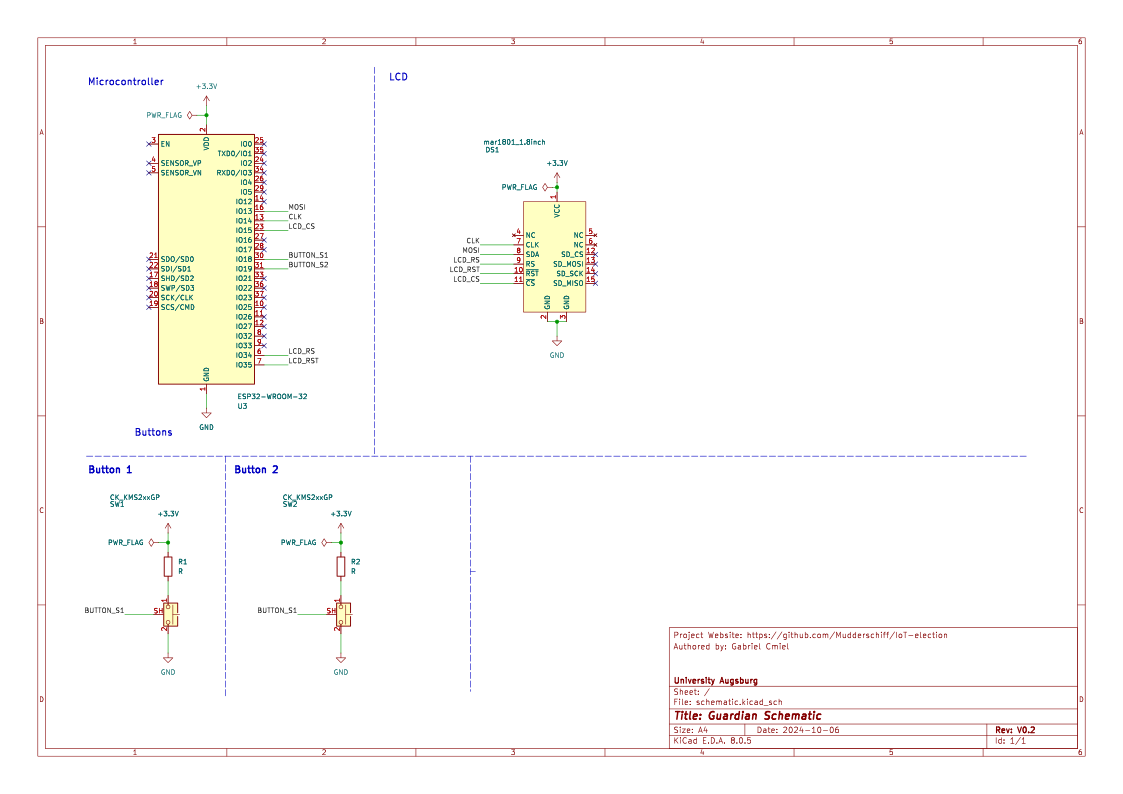
\includegraphics[scale=.5]{abbildungen/schematic.png}
	\caption{Schematic of the Guardian Prototype}\label{Fig:schematic} 
\end{figure}

As shown in Table \ref{tab:basic-component-list}, the hardware components used in our prototype include a ESP32 development board, an LCD display module, jumper wires, breadboard and a module with 2 Buttons. The connectivity of these components are shown in the schematic in Figure \ref{Fig:schematic}. The NodeMCU ESP32 development board is used as the Main Controller. The LCD display module is used to display information to the user. The button module is used to interact with the user. The jumper wires are used to connect the components. The breadboard is used to build the circuits.

\subsection{NodeMCU ESP32 Development Board}
The NodeMCU ESP32 development board is equipped with the ESP32-WROOM-32 module. 

\begin{comment}

\subsection{1,8" LCD Display Module}
The 1,8" LCD Display Module has a resolution of 128x160 Pixels and is equipped with a ST7735R Display Driver.  The module also contains a microSD Slot which won't be used in this project \cite[2]{lcd}.

\subsection{Button Module}
The Button Module is an integrated circuit that features 2 buttons and integrated pull-up resistors. \cite[1]{button-ds}

\section{Python Client}
Our python client imports the python package ElectionGuard \cite{python-reference}. The ElectionGuard Python package is a reference implementation of the ElectionGuard 1.0 specification. It covers the entire suite of functionality required to implement an end-to-end verifiable election as part of a voting system \cite{eg-docs}. 



In the proposed voting system the python client will act as the administrator, the ballot box and the encryption device of the election. Administrating the election requires loading and semantically verifiying the Election manifest before the election.





Before the election the python client load the Election Manifest for our election and semantically checks the data format required to conduct an ElectionGuard Election. 




The python client loads the manifest file used for our election. In ElectionGuard an election manifest has to be semantically checked against the data format required to conduct an ElectionGuard Election. 


The python client then generates the election keys and the election context. The election keys are used to encrypt the ballots and the election context is used to verify the election. The python client then encrypts the ballots and generates the proofs of the encryption. The encrypted ballots and the proofs are then sent to the ESP32. The ESP32 decrypts the ballots and verifies the proofs. The ESP32 then generates the proofs of the decryption and sends them back to the python client. The python client then verifies the proofs of the decryption and generates the proofs of the election. The proofs of the election are then sent to the ESP32. The ESP32 verifies the proofs of the election and sends the results back to the python client. The python client then verifies the results and outputs the final results of the election.

The tasks of the python client can be divided into three stages pre-election, intra-election and post-election.







The python client loads the manifest file used for our election. In ElectionGuard an election manifest has to be semantically checked against the data fromat required to conduct an ElectionGuard Election.



Espressif IoT Development Framework (ESP-IDF) is a software development framework intended for the development of Internet-of-Things (IoT) applications for the ESP32 board \cite{esp-prog}. ESP-IDF consists of components written specifically for ESP-IDF as well as third-party libraries.\cite{esp-prog} For example, the real-time operating system kernel used for ESP-IDF applications is the third-party component called FreeRTOS \cite{esp-prog}. ESP-IDF projects use the same componment based approach and can be seen as an amalgamation of a number of components \cite{esp-prog}.
\end{comment}

\begin{figure}
	\centering
	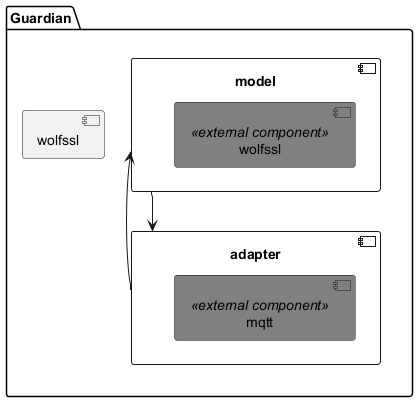
\includegraphics[width=1\textwidth]{abbildungen/Diagramme/components.png}
	\caption{}
	\label{Fig:uml-classes-python}
\end{figure}


\section{Computation}
ElectionGuard uses integer ElGamal cryptography within its specific cryptographic operations. The system performs four key operations on very large integer values: \textbf{modular exponentiation}, \textbf{modular multiplication}, \textbf{modular addition}, and \textbf{SHA-256} hash computation. To handle the large integer values involved in these operations, specialized libraries for large integers may be employed, or the operations can be developed from scratch \cite[21, 25-26]{eg-spec}. When developing these modular operations from the ground up, it is common for intermediate values to become excessively large. Techniques such as modular reduction are often necessary to ensure that values remain manageable \cite[21, 25-26]{eg-spec}.Consequently, employing optimized libraries for modular arithmetic becomes crucial for achieving good performance \cite[22]{eg-paper}.

\subsection{Cryptographic constants}
Among all computations in ElectionGuard, modular exponentiation presents the highest computational cost, serving as the primary limiting factor in performance analysis \cite[22]{eg-spec}. Within ElectionGuard, most modular exponentiation operations utilize a fixed base, which may be either the generator (g) or a public key \cite[22]{eg-paper}. The generator G is a mathematical constant specified in the ElectionGuard specification.

The standard baseline parameters include:
\begin{itemize}
    \item A 4096-bit prime (p) \cite[22]{eg-spec}
    \item A 4096-bit generator (g) \cite[23]{eg-spec}
    \item A 256-bit prime (q) \cite[21]{eg-spec}
\end{itemize}

Alternatively, the system can also utilize reduced baseline parameters, which consist of:
\begin{itemize}
    \item A 3072-bit prime (p) \cite[36]{eg-spec}
    \item A 3072-bit generator (g) \cite[36-37]{eg-spec}
    \item A 256-bit prime (q) \cite[36]{eg-spec}
\end{itemize}

For this application, we opt for the reduced parameters, as they offer enhanced performance, albeit at the expense of lower security \cite[36-37]{eg-spec}. The cryptographic constants used in the implementation can be found in Appendix \ref{lst:constants}.



\subsection{Comparison of ElectionGuard Implementations}
The Python reference implementation of ElectionGuard utilizes the C-coded Gmpy2 library for large integer arithmetic. In contrast the C++ and Kotlin implementations rely on the HACL* C library for similar purposes \cite{eg-docs}. Interestingly, both implementation use C-coded libraries for handling large integer arithmetic. Moreover, the C++ implementation incorporates pre-computed tables to speed up certain modular exponentiations \cite{eg-docs}. This optimization is possible because many of the exponentiations are performed with a fixed base, either the constant generator (g) or a public key. The pre-computed tables contain specific powers of these bases \cite{eg-docs}.

\subsubsection{Feasability of the Python reference on ESP32}
The Python reference implementation encompasses the entire ElectionGuard specification \cite{python-reference}. Running the Python reference implementation on the ESP32 may be achievable through \textbf{MicroPython}, an implementation of Python 3.x targeted for microcontrollers and embedded systems. MicroPython mirrors and adapts the functionalities of the standard Python library to accommodate the limitations inherent to to microcontrollers, such as restricted memory and processing speed \cite{micropython} \cite[234]{micropython-performance}. There are drawbacks to this approach, as certain essential modules, functions, and classes may be absent in MicroPython \cite{micropython}. Additionally, applications developed in MicroPython are prone to memory fragmentation and may experience issues with objective expending in size. \cite[234]{micropython-performance}. Depending on the complexity of the task and memory allocation, the performance of MicroPython might be inferior to that of a C implementation \cite[237]{micropython-performance}. For instance, in a comparative study of software-based SHA-256 computation for the ESP32, the C implementation outperformed the MicroPython implementation by 45\% \cite[237]{micropython-performance}.

\subsubsection{Feasability of the C++ reference on ESP32}
The ElectionGuard C++ reference implements only a subset of the ElectionGuard specification, focusing on the encryption library and thus addressing only intra-election functionalities cite{cpp-reference}. ESP-IDF supports the development of applications in C++. Certain C++ features, such as exception handling, must be enabled in the project configuration. This results in a slight increase in the application binary size \cite{esp-prog}. The Runtime Type Information (RTTI) feature can remain disabled since dynamic cast conversions and the typeid operator are not utilized in the ElectionGuard C++ implementation. C++ Threads are supported, these are implemented as wrappers around C pthreads, which in turn wrap around FreeRTOS tasks \cite{esp-prog}.

Upon porting the C++ implementation to an ESP32 component, we conducted tests using the provided C Unit Tests, particularly focusing on the ElGamal encryption test. However, the test failed upon invoking the \textbf{pow\_mod\_p()} function, which is intended to optimize modular exponentiation by utilizing pre-computed tables.

\begin{lstlisting}[language=C++, caption={FixedBaseTable Definition}]
    typedef std::array<std::array<uint64_t[MAX_P_LEN], OrderBits>, TableLength> FixedBaseTable;
\end{lstlisting}

The \textbf{FixedBaseTable} is defined as a 2D array. Here, \textbf{MAX\_P\_LEN} denotes the lenght of each \textbf{uint64\_t} array, \textbf{OrderBits} indicates the number of \textbf{uint64\_t} arrays in each inner array, and \textbf{TableLength} represents the number of inner arrays in the outer array.

The \textbf{pow\_mod\_p()} function is optimized for specific parameters: ( order\_bits = 256 ), ( window\_size = 8 ), and ( table\_length = 32 ). Any modifications to these parameters could affect the function's internal operations. The window\_size determines into how many groups of (k) bits the exponent is parsed, while the order\_bits reflect the number of possible values within each group. With an 8-bit window\_size, the order\_bits would amount to 256 (2^8) \cite[22]{eg-spec}.

To estimate the memory requirements of the \textbf{FixedBaseTable}, we can calculate the total size in bytes as follows:	

\begin{equation}
    \mathrm{FixedBaseTable Size} = \mathrm{sizeof(uint64\_t)} \times \mathrm{MAX\_P\_LEN} \times \mathrm{OrderBits} \times \mathrm{TableLength}
\end{equation}

Given that \textbf{MAX\_P\_LEN} is defined as 64, substituting into the equation yields a total size of 4MB:

\begin{equation}
    \mathrm{FixedBaseTable Size} = 8 \times 64 \times 256 \times 32 = 4194304 \mathrm{ bytes} = 4 \mathrm{ MB}
\end{equation}

If we calculate the size of the \textbf{FixedBaseTable} with our reduced baseline parameters, we find:

\begin{equation}
    \mathrm{FixedBaseTable Size} = 8 \times 48 \times 256 \times 32 =  3145728 \mathrm{ bytes} = 3 \mathrm{ MB}
\end{equation}

The ESP32 features (320 KB) of DRAM. Due to a technical limitation, a maximum of (160 KB) is available for dynamic allocation \cite{esp32-ref}. Consequently, the \textbf{FixedBaseTable} exceeds the memory capacity of the ESP32. While reducing the \textbf{window\_size} results in smaller tables and reduced memory usage, it simultaneously increases the number of multiplications \cite[22]{eg-spec}. Considering these resource limitations and the fact that the ElectionGuard C++ implementation is designed with Intel Atom-level processor performance in mind, alongside the memory requirements of the \textbf{FixedBaseTable} optimization, it becomes evident that the C++ implementation is not feasible on the ESP32 \cite{eg-docs}.

\subsection{Implementation Strategy for ESP32}
As previously discussed, both the Python and C++ reference implementations prove impractical for porting to the ESP32. While the Python implementation may be feasible with MicroPython, the performance may be suboptimal due to possible memory fragmentation. The C++ implementation, on the other hand, is not viable due to memory and processor constraints. Ultimatelty, a pure C implementation stands out as the most feasible approach for the ESP32. To achieve optimal performance on the ESP32, we must consider the dedicated hardware accelerators available. The ESP32 supports several cryptographic hardware acceleration capabilities including AES, SHA, RSA, and RNG as illustrated in the functional block diagram \ref{Fig:esp32-crypto}. These hardware accelerators significantly enhance operational speed and reduce software complexity for the aforementioned cryptographic primitives \cite[32]{esp32-series}. 

In ESP32 the cryptographic primitives are implemented in a fork of the mbedTLS library. The fork includes patches related to hardware routines for on-board cryptographic hardware acceleration \cite{esp32-ref}. Optionally, a port of the WolfSSL library is also available, which also includes ESP32-specific hardware routines \cite[114]{wolfSSL-manual}. To sucessfully run WolfSSL on the memory-restricted ESP32, it is essential to configure the component to use less memory, albeit at a potential performance cost. An excerpt from the Component configurations for WolfSSL can be found in Appendix \ref{lst:user_settings}

\subsection{\ac{RNG}}
In the context of ElectionGuard, generating random values is crucial for various operations, including the generation of private keys and the use of nonces in various proofs \cite[9, 13]{eg-spec}. The ESP32 features a True Random Number Generator \ac{TRNG} that can produce 32-bit random numbers that are suitable for cryptographic purposes. Unlike Deterministic Random Bit Generators \ac{DRBG}, which rely on algorithms to produce random numbers, the ESP32's \ac{TRNG} generates randomness from physical processes. This includes leveraging thermal noise and asynchronous clock mismatches, ensuring a high level of unpredictability, essential for cryptographic operations \cite[604]{esp32-ref}.

To utilize the \ac{TRNG} effectively, it is necessary to enable a source for thermal noise; otherwise, the \ac{TRNG} will return pseudo-random number \cite[609]{esp32-ref}. The High-speed ADC is enabled automatically when the Wi-Fi or Bluetooth module is enabled, which is the case in our design \cite[610]{esp32-ref}. When the noise is sourced from the high-speed ADC, it is advisable to read the \textbf{RNG\_DATA\_REG} register at a maximum rate of 5 MHz \cite[609]{esp32-ref}. However, the values from the high-speed ADC can be saturated in extreme cases, leading to lower entropy. It is advisable to enable the SAR\_ADC as a secondary noise source. The \textbf{RNG\_DATA\_REG} register should then be read at a maximum rate of 500 kHz to obtain the maximum entropy \cite[609]{esp32-ref}.

In our ESP32 implementation, as outlined in Appendix \ref{lst:rng}, we aim to generate random values below a specific mathematical constant (q), which is a 256-bit prime number. To achieve this objective, we fill a buffer with 256-bits of randomness utilizing the system API function esp\_fill\_random(). To ensure that the generated 256-bit number does not exceed (q), we perform a modulo operation with the value of (q). To obtain a 256-bit number, esp\_fill\_random() reads the 32-bit RNG\_DATA\_REG register eight times. The function will busy-wait if the reading frequency exceeds acceptable limits \cite{esp32-ref}.This limitation arises because the function must ensure that sufficient external entropy has been introduced into the hardware RNG state. For our use case the function should not delay. If the function delays, we should consider using a strong software \ac{DRBG} such as mbedTLS CTR-DRBG, mbedTLS HMAC-DRBG, or WolfSSL DRBG, which can be initialized with the TRNG values as a seed \cite{esp32-ref} \cite[588]{wolfSSL-manual}.



\subsection{\ac{SHA} Accelerator}
ElectionGuard encrypts non-vote data, such as cryptographic shares of a guardian’s private key, using hashed ElGamal encryption. This method employs a key derivation function \ac{KDF} to generate a key stream that is XORed with the data. The Keyed-Hash Message Authentication Code \ac{HMAC} is used for message authentication and is integral to the implementation of the \ac{KDF}. In ElectionGuard, HMAC is instantiated as HMAC-SHA-256, which uses the SHA-256 function \cite[7]{eg-spec}. An implementation of the HMAC-SHA-256 function can be found in Appendix \ref{lst.get_hmac}. 

The SHA-256 hash function is frequently applied in various cryptographic operations within ElectionGuard, with implementation details provided in Appendix \ref{lst:hash}. The ESP32 microcontroller is equipeed with a \ac{SHA} Accelerator that significantly enhances the performance of\ac{SHA} operations compared to purely software implementations \cite[589]{esp32-ref}. Notably, this accelerator supports the SHA-256 algorithm used in ElectionGuard. However, it processes only one message block at a time and does not handle padding operations. Therefore, software must manage the division of longer messages into 512-bit blocks, along with any required padding \cite[2]{esp32-series}. 

In multi-core environments, libraries like mbedTLS and WolfSSL implement fallback mechanisms to software implementations when multiple concurrent hashing operations are initiated. As a result, simultaneous computations revert to software calculations \cite{mbedTLS-fork} \cite{wolfSSL-port}. Benchmarks uzilizing mbedTLS at processor speeds of 240 MHz reveal that hardware acceleration achieves performance nearly three times faster than software couterparts \cite[41-42]{eval-crypto}. When using the WolfSSL library with the fastmath library, benchmarks indicate that the \ac{SHA} Accelerator operates more than eight times faster than its software counterpart. Thus, the \ac{SHA} Accelerator is an effective solution for speeding up SHA-256 hashing operations on the ESP32.

\begin{comment}
    The 1.0 specification of ElectionGuard has under-specification on how inputs to the cryptographic hash function should be serialized. This leads to compability issues between different implementations \cite[23-24]{eg-paper}.
\end{comment}

\subsection{\ac{RSA} Accelerator}
\begin{comment}
        Fundamentally, ElectionGuard encryption is a CPU-bound operation \cite[24]{eg-paper}
\end{comment}

ElectionGuard's decision to use integer ElGamal instead of elliptic-curve ElGamal was driven by its conceptual simplicity and lower implementation barrier \cite[7]{eg-paper}. While elliptic-curve cryptographic \ac{ECC} techniques offer computational advantages, such as reduced computing requirements and smaller key sizes for the same security level \cite[1, 6]{ecc-eval}, the integer ElGamal approach aligns well with the ESP32 hardware. This is because the RSA algorithm, like integer ElGamal, relies on large integer arithmetic. Specifically, the ESP32 chip supports independent arithmetic operations, including large-number multiplication, large-number modular multiplication, and large-number modular exponentiation \cite[32]{esp32-series} \cite[603]{esp32-ref}. Consequently, the RSA Accelerator can accelerate two key operations: modular multiplication and the computationally intensive modular exponentiation. However, modular addition cannot be accelerated using dedicated hardware and must rely on a software implementation.


The RSA Accelerator supports eight operand lengths for modular exponentiation and modular multiplication, including the reduced 3072-bit and even the 4096-bit baseline parameters used in our implementation \cite[598]{esp32-ref}. The large-number modular exponentiation operation computes \( Z = X^Y \mod M \), while the large-number modular multiplication operation computes \( Z = X \times Y \mod M \). Both operations are based on Montgomery multiplication. In addition to the input arguments \( X \), \( Y \), and \( M \), two additional arguments are required: the Montgomery Inverse \( \overline{r} \) and the inverse of \( M' \). These additional arguments are precomputed by software \cite[598-599]{esp32-ref}.

The wolfSSL library defaults to a software implementation for smaller operands, whereas the mbedTLS library lacks such a fallback mechanism. Interestingly, using hardware acceleration for small operands can be less efficient than a software implementation. For example, in one test, the mbedTLS modular exponentiation function with hardware acceleration was 1.44 times slower for small operands but 12.84 times faster for large operands \cite[51]{eval-crypto}. This inefficiency for small operands likely stems from the initialization overhead of the hardware accelerator, which outweighs the benefits for smaller values. However, the mbedTLS library provides functions that allow caching of the \( \overline{r} \)-inverse and \( M' \)-inverse values, which can significantly speed up operations \cite[51]{eval-crypto}. Since calculating the \( \overline{r} \)-inverse is computationally expensive, precomputing and caching these values can enhance performance \cite[51]{eval-crypto}.

In our implementation, the modular exponentiation function switches to a software implementation for small values, as shown in Appendix \ref{lst:modular_exp}. This switch occurs during polynomial calculations, where the number of polynomials (starting from 0 and incrementing) is used as the exponent in the modular exponentiation operation. The polynomial function is detailed in Appendix \ref{lst:compute_polynomial}.

In summary, the RSA Accelerator effectively accelerates modular exponentiation and modular multiplication in the ElectionGuard implementation. The mbedTLS library offers efficiency gains through caching of the \( \overline{r} \)-inverse and \( M' \)-inverse values. However, its lack of a fallback mechanism for small operands necessitates an additional software implementation to avoid inefficiencies when using the RSA Accelerator with small values.


\begin{comment}
    Single Factroy App (large) no OTA
    Remalloc/CMALLOC
    MQTT5 NoLocal not supported
    MQTT Buffer size changed
\end{comment}




\section{Communication}
\begin{figure}[ht]
    \centering
    \begin{subfigure}[b]{\textwidth}
        \centering
        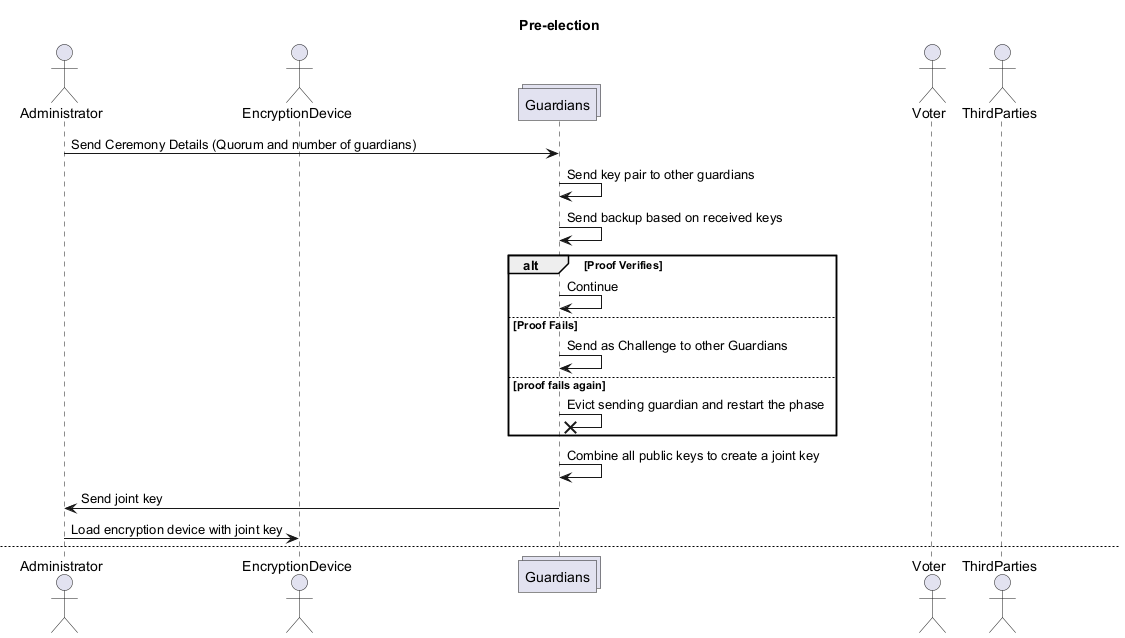
\includegraphics[width=\textwidth]{abbildungen/Diagramme/communication-seq.png}
        \caption{Communication Sequence in the Pre-election phase}
        \label{Fig:comm-pre}
    \end{subfigure}
    \hfill
    \begin{subfigure}[b]{\textwidth}
        \centering
        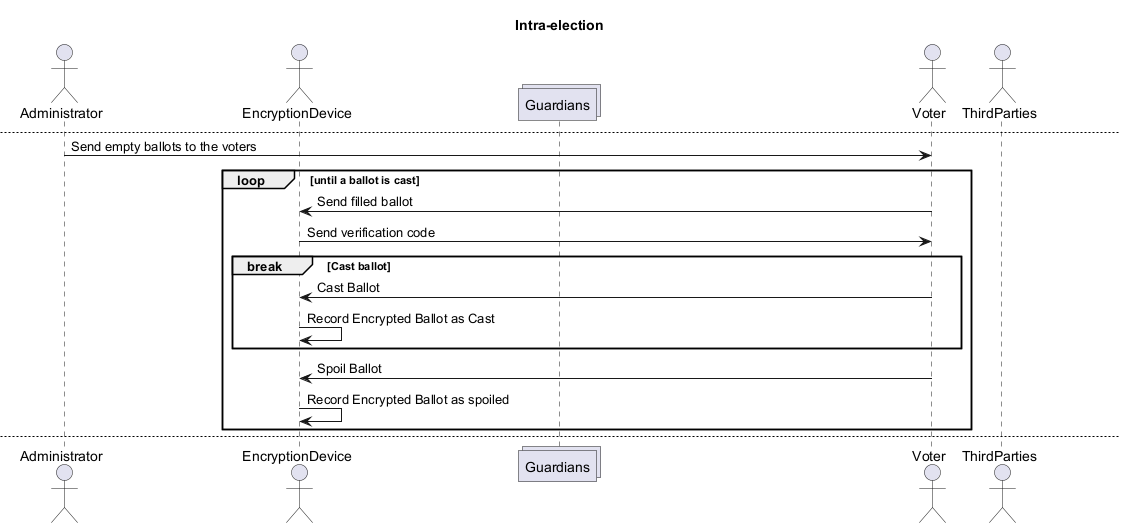
\includegraphics[width=\textwidth]{abbildungen/Diagramme/communication-seq_001.png}
        \caption{Communication Sequence in the Intra-election phase}
        \label{Fig:comm-intra}
    \end{subfigure}
    \hfill
    \begin{subfigure}[b]{\textwidth}
        \centering
        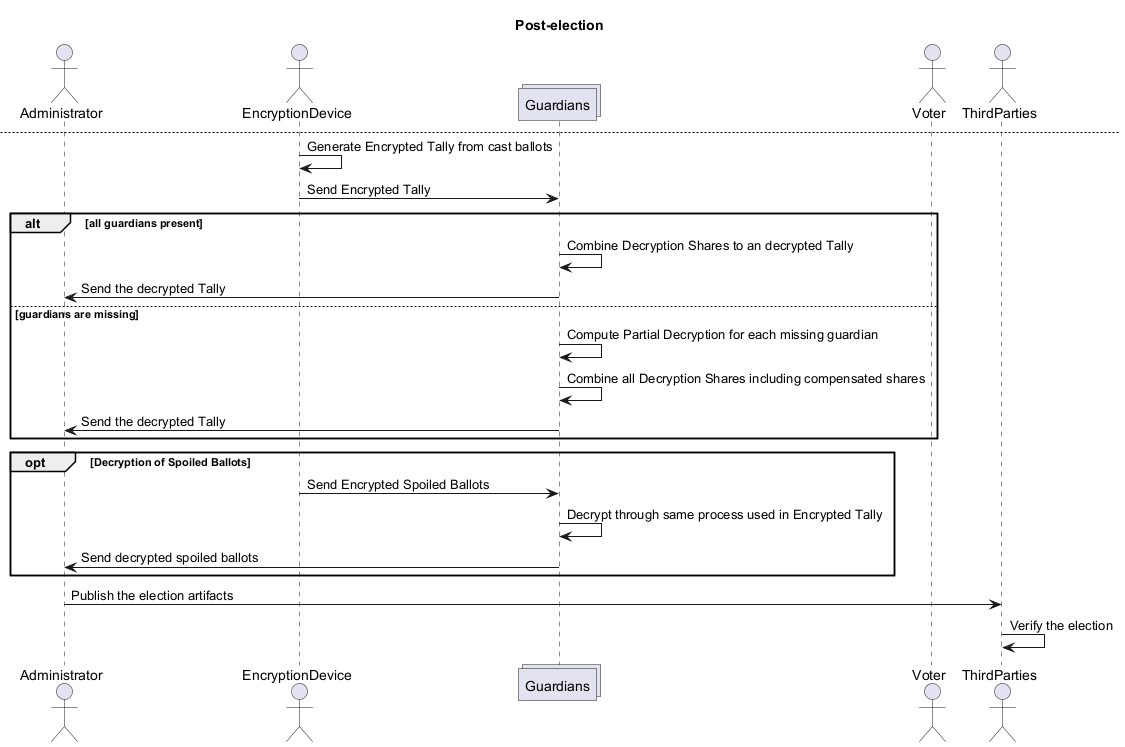
\includegraphics[width=\textwidth]{abbildungen/Diagramme/communication-seq_002.png}
        \caption{Communication Sequence in the Post-election phase}
        \label{Fig:comm-post}
    \end{subfigure}
    \caption{Communication Sequence}
    \label{fig:comm-seq}
\end{figure}

A sequence diagram of the pre-election steps are seen in \ref{Fig:comm-pre}. In it we see that the Election administrator sends ceremony details to the Guardians and receives a joint key in return. The joint key is then loaded into the encryption devices. In order to generate a joint key each guardian send their public key to a receiving guardians. The receiving guardian generates a designated backup for each guardian. If a guardian receives a designated backup the included proofs are verified. If a proof failed the guardian send the unverified backup to other guardians as a challenge. If the proof fails again this guardian that generated the backup is evicted and the ceremony has to be restarted. 

A sequence diagram of the intra-election steps is seen in \ref{Fig:comm-intra}. The election administrator would need an empty ballot to the voter. A voter then sends their filled ballot to the encryption device. The encryption devices sends back a verification code. The voter can then decide to either cast or spoil the ballot associated with the verification code. If the voter decides to spoil the ballot the encryption devices needs to mark the encrypted ballot as spoiled and the process starts a new. The loop is broken if the voter decides to cast a ballot.

In the post-election steps the encryption device generates a decrypted tally from all cast encrypted ballots and send the encrypted tally to the guardians. If all guardians are present each guardian generates a decryption share which is combined to a decrypted tally. This decrypted tally is then send back to the administrator. If guardians are missing the guardians in addition to generating their decryption share have to compensate for the missing guardians. Missing decryption shares are reconstructed from the backups generated in the pre-election phase. Finally all decryption shares including the reconstructed shares are combined into a decrypted tally. The decrypted tally is then send back to the administrator. Optionally the spoiled ballots can be decrypted through the same mechanisms as the encrypted tally. At the end of the election the administratir publishes all election artifacts to the public for scrutiny.


IoT systems rely primarily on using messaging protocols for exchanging
IoT data and there exists several protocols or frameworks that support distinct types of messaging patterns 
Given that IoT devices typically have limited computational resources and processing power, choosing a
lightweight, reliable, scalable, interoperable, extensible and secure messaging protocol becomes a very
challenging task. \cite[1]{protocols}.


\subsection{Data Scheme}

\subsection{Data Link Layer Protocols}
When choosing a suitable messaging protocol, it is imperative to consider the hardware characteristics of IoT devices and type of data link layer protocols employed \cite[1-2]{protocols}. The data link layer is responsible for data transfers between network entities \cite[3]{protocols}. The ESP32 supports Wi-Fi and Bluetooth data link layer protocols. The Bluetooth system on the ESP32 can be further divided into Classic Bluetooth and \ac{BLE} \cite{esp-prog} \cite{esp-faq}. Both Wi-Fi and Bluetooth can coexist but would require time sharing control \cite{esp-faq}.

Wi-Fi (802.11n) generally has a higher transmission range of approximately 1 km compared to \ac{BLE}, which has a range of approximately 100 m \cite[3]{protocols}. The transmission throughput of WiFi is generally higher compared to the transmission throughout of \ac{BLE} \cite[3]{protocols}. However, IoT devices can vary significantly in terms of the bandwidth they support. IoT devices do not use a universal radio technology, and therefore, the physical data rate they support varies considerably depending on the size and hardware components used to build these devices \cite[1-2]{protocols}. The throughput additionaly depends on various factors such as environmental interference, connection interval, and MTU size. The maximum \ac{BLE} throughput achievable on the ESP32 is about 90 KB/s, for Classic Bluetooth is about 200 KB/s, and for Wi-Fi it is about 20 MBit/s TCP and 30 MBits/ UDP \cite{esp-prog} \cite{esp-faq}.

In addition to these data link layer protocols, there are also a plethora of custom protocols at the data link layer. The Wi-Fi and \ac{BLE} stacks also support Mesh Networking, which enables many-to-many device communications and is optimized for creating large-scale device networks \cite{esp-prog}. The Wi-Fi stack additionally supports Wi-Fi Neighbor Awareness Networking (NAN), which allows device-to-device communication directly between two devices. The ESP32 also supports the proprietary protocol ESP-NOW, which allows for connectionless device-to-device communication between ESP32 devices \cite{esp-prog}. 

Understanding protocols at the data link layer is not sufficient to build IoT applications. It is essential to also consider protocols that exist at the application level, complementing those at the data link layer \cite[2]{protocols}. Carefully choosing a protocol closer to the application layer while also considering crucial system requirements such as Quality of Service, bandwidth, interoperability, and security becomes inevitable \cite[2]{protocols}.

\subsection{Application Layer Protocols}
When developing IoT systems, choosing the most appropriate
Messaging Protocols becomes a challenging task \cite[2]{protocols}. Although all messaging protocols are used for data communication between two or more entities via some transmission medium, some of the characteristics of each
protocol vary \cite[15]{protocols}. To identify a suitable protocol requires sufficient background knowledge on how these protocols operate and how to overcome challenges that may arise \cite[2, 15]{protocols}. A suitable messaging protocol helps reduce network traffic and latency and thus increases an IoT application's reliability \cite[2]{protocols}. For example, using application layer protocols that are capable of capturing data much faster than actual physical data rates often leads to high latency. Therefore, it would be desirable when developing IoT applications to consider messaging protocols that can accommodate or support physical data rates at the data link layer \cite[2]{protocols}. 

The application layer is an abstraction layer \cite[3]{protocols}. Within ESP32 exists several application layer protocols that address a wide range of application requirements.  Each of these protocols provide various features that vary in terms of reliability, quality of service, performance, functionality and scalability, among other factors. \cite[3]{protocols}. Some of the protocols that exist as components of the ESP32 at the application layer include: HyperText Transfer Protocol (HTTP), Secure HTTP (HTTPS), Message Queueing Telemetry Transport (MQTT) over TCP, MQTT over Websocket \cite{esp-prog}. In addition, industry specific protocols used primarily in industrial IoT environments also exist such as Modbus \cite[3]{protocols}. And ESP32 also provides support for the proprietary protocol ESP-NOW \cite{esp-prog}.

Choosing an appropriate messaging protocol depends on a number of factors including IoT application's software capabilities, device or hardware capabilities, and average size of data exchanges, among many others. \cite[2]{protocols}.

ESP32-Now has a communication scope of device-to-device communication meaning we could use this protocol for the communication between ESP32 devices. A communication between Guardians during the key exchange would thus be possible however the communication between the Election Administrator and the Guardians would not be possible. The communication between Guardian is also not suitable. ESP-Now limits the data payload to 250 bytes \cite{esp-prog}. This is unstuitable considering that sending a single public key is already 384 bytes (3072 bit key).

\begin{figure}
    \centering
    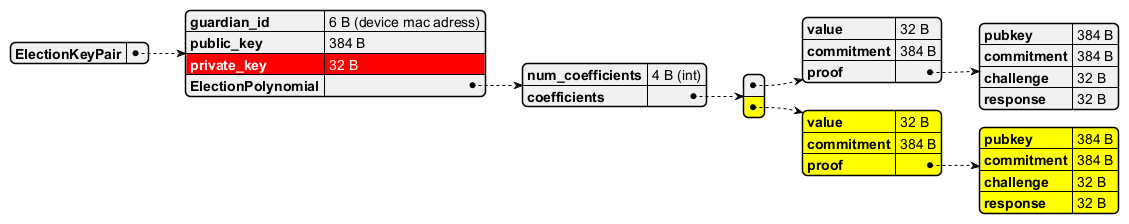
\includegraphics[width=1\textwidth]{abbildungen/Diagramme/mElectionKeyPair.png}
    \caption{Key Pair message size}
    \label{Fig:keypair-size}
\end{figure}

The maximum packet size for ESP BLE Mesh transmission is 384 bytes \cite{esp-faq}. And the maximum packet size for Wi-Fi Mesh data transmission is 1,456 bytes. \cite{esp-faq}. The Wi-Fi Mesh data transmission rate is also too small. The minimum package size for a public key without any additional coefficients (yellow) and without the private key (red) send by a guardian is 1642 bytes. The message scheme is seen in figure. \ref{Fig:keypair-size}. Each additional coefficients adds 1248 bytes to the message. This is largely due to large commitment sizes. MQTT has a maximum payload size of 256 MB and HTTP does not define a maximum message size. The message size is thus not a limiting factor for MQTT and HTTP protocols.

HTTP is an generic, stateless request-response protocol in which a
client sends a request message and a server generates a response message  \cite[8]{protocols}. Inside our network we would need to utilize something like multicast DNS (mDNS) for example in order to discover the services in our network (e.g. other guardians or the election administrator). \cite[20]{protocols}


Message reliability is imperative in this publish-
subscribe brokering model. That is, an IoT system may
require that messages be delivered in a reliable manner
where all clients acknowledge the receipt of these messages.
MQTT supports a Quality of Service (QoS) level when
messages are published through the Connect Flags of the
Fixed Header using the Will QoS parameter (bits 4 and 3).
These bits specify the QoS level applied when a broker
publishes a message to one or more clients. MQTT supports
three levels of QoS as presented in Table VI.
\cite[11]{protocols}
As shown in Table VI, as the QoS level increases, the
reliability of messages’ delivery also increases. However,
this also increases the overhead associated with ensuring that
all clients receive the intended messages. The more clients
are subscribed to receive a message with QoS 2, for example,
will increase the overhead on the message broker while
ensuring the delivery of the message without duplication or
retransmission.
\cite[11]{protocols}
The MQTT handling of disallowed Unicode code points
provides a client or server the option to decide on the
validation of these code points (e.g. UTF-8 encoded strings).
As a result, an endpoint does not necessarily need to validate
UTF-8 encoded strings (e.g. topic name or property). As
such, a client could potentially use this as a vulnerability and
causes a subscribed client to close the network connection
using a topic that contains an invalid Unicode code point. A
malicious client can then use this as a security exploit for
possibly causing a Denial of Service (DoS) attack.
Therefore, enabling UTF-8 encoded strings, for example,
can allow these security exploits to occur in cases they are
used as control characters or in control packets (see the first
\cite[11]{protocols}

QoS 0 lowest
at most once delivery
- no response is sent by receiver, no retry is performed by sender
- message arrives at the receiver either once or not at all
QoS 1 medium
at least once delivery
- ensures that a message arrives at the receiver at least once
- receiver may send further PUBLISH packets while waiting to receive acknowledgments
QoS 2 highest
exactly once delivery
- ensures that a message arrives at the receiver exactly once without duplication
- increased overhead associated with this level
\cite[11]{protocols}

\subsection{MQTT's role in IoT}
MQTT is an asynchronous lightweight publish/subscribe messaging protocol designed for Machine-to-Machine (M2M) communication \cite[2]{protocols}. It is designed to handle situations in case of unreliable networks or intermittent connectivity, and enables the exchange of data in a real-time manner \cite[10]{protocols}. 

MQTT is composed of a broker and clients establish a connection with the
broker at any time. In this model, clients send messages through the broker which is known as the publisher. Then, the broker filters these incoming messages and distributes them to clients who are interested in receiving these messages. To this extent, a client that registers with the broker to receive these messages must first subscribe to specific topics. Clients receive the payload when a new device publishes a message. A subscriber can receive a published message later. That is, the subscribers can receive published messages at different times. In this publish-subscribe model, a publisher can send messages to a number of subscribers with one single publish
operation to the broker. The broker handles the "broadcasting" or sending messages to all subscribers subscribed to topic of the message 

Figure 9
presents a high-level overview of the MQTT brokering
model that shows all of the entities involved in this
architecture including: (a) centralized broker, (b) publishers
and (c) subscribers.  \cite[10]{protocols}
as shown in Figure 9.


There are a number of MQTT model implementations
including Mosquitto, eMQTT, HiveMQ, Moquette, among
many others. \cite[10]{protocols}



For MQTT dicovery is based on topics \cite[27]{protocols}

\subsection{Comparison MQTT vs HTTP}

MQTT is considered lighter than HTTP 1.1 and supports
a near real-time message exchange  \cite[10]{protocols}

HTTP may not be an ideal choice for a messaging protocol for data connectivity \cite[15]{protocols}. 


Furthermore, when choosing a message protocol such as
MQTT, the number of message transmissions increases
significantly as more clients subscribe to topics.
\cite[19]{protocols}

The case
can become worse if the broker’s resources are maximized
and hence a broker becomes a source for a Single Point of
Failure (SPoF). Because MQTT is designed primarily for a
Device-to-Cloud (D2C) communication scope, the problem
of SPoF can be resolved by serverless computing which
increases the agility of the deployed IoT application
\cite[19]{protocols}


MQTT is D2C communication scope, the
further these nodes are from the deployed serverless solution
in terms of distance, the longer is the travel time of the MQTT
messages and the higher the latency \cite[20]{protocols}

However, existing implementations of MQTT vary in
terms of performance and scalability. In [111], the authors
compared Mosquitto, HiveMQ and BevyWise MQTT broker
deployed on the cloud
\cite[20]{protocols}

There are a number of studies that have examined the
performance and scalability of communication protocols.
Some studies have found that the throughput in MQTT drops
significantly as the number of clients’ subscriptions increases
[112, 113]. In [114], the authors compared the performance
of DDS and MQTT. \cite[21]{protocols}

The performance and scalability of messaging protocols
vary. CoAP and HTTP have an additional overhead
associated with transporting messages. CoAP and HTTP
should be used in cases where low latency is not of critical
importance. Hence, this makes these two protocols not very
suitable for real-time IoT edge- or fog-based systems. MQTT
follows a device-to-cloud data flow and therefore introduces
network latency dependent on the cloud service performance.
\cite[21]{protocols}

Generally, message brokers may deliver 100 to 1000
messages per second per subscriber [20, 117]. However, these
messaging brokers can vary significantly.

esults in Section V.D which
suggested that the performance of MQTT in terms of latency
degrades significantly as the number of messages increases. 
\cite[22]{protocols}

In addition, MQTT used
the least power consumption in delivering large volumes of
messages compared to CoAP and HTTP. \cite[22]{protocols}

 MQTT had the least power consumption in
terms of battery life followed by CoAP and then HTTP. That
is, HTTP had 5.3 times the power consumption of that of MQTT and 2.8 times the power consumption of that of CoAP \cite[23]{protocols}

Furthermore,
IoT devices are generally used by humans which makes them
vulnerable to intruders that attempt to gain unsolicited access
or collect confidential personal data in a malicious manner.
\cite[23]{protocols}

An IoT
communication protocol needs to ensure that only authorized
users regardless if they are publishers or subscribers
Furthermore, such vulnerabilities may occur when
offering QoS level 2 which may explain why many IoT cloud
providers not to provide support at this level as presented in
Table VII. 
Although each protocol provides different levels of
security measure\cite[23]{protocols}

Although HTTP remains to be among the top two
protocols across all years, there is an apparent drop in its
usage with approximately 9% decrease in 2018 as illustrated
in Figure 21. On the contrary, MQTT has witnessed a
significant increase in its usage from 2017 to 2018. The
survey results from the 2019 Eclipse Foundation and Eclipse
IoT Working Group is partial but report that HTTP and
MQTT remain among the top three messaging protocols
[156]. In addition, the AMQP protocol has been witnessing
a gradual increase over the years in terms of its usage by
developers who have completed the surveys and as illustrated
in Figure 21. DDS remains steady at the same rate while
CoAP has witnessed a slight decline between 2017 and 2018.
In the results from the 2019 survey, the report show that
CoAP has dropped below a 15% response rate.
\cite[26]{protocols}


HTTP
Advantages:
 uses a push approach which involves a persistent
connection between client and server
Disadvantages:
 header size is large: this adds processing overhead for
devices particularly constrained IoT devices
 high network latency: this makes the protocol not
suitable for real-time or mission-critical IoT systems
 uses text not binary encoding
 protocol does not provide any QoS support
 protocol is not easily scalable
 computational overhead due to encrypting and
decrypting (secure) messages
\cite[26]{protocols}

MQTT
Advantages:
 has a transient data message transmission cycle
 good for cloud-based IoT applications (D2C)
 a lightweight protocol and works fairly well over
constrained networks
 provides an adequate level of QoS support (0, 1, 2)
 protocol supports asynchronous messaging
 protocol is an event-driven which enables an IoT
system to scale up (or down)
 protocol can be used for M2M communication
 supported by many IoT cloud providers (Table III)
Disadvantages:
 does not support large payloads
 topic names are often long; inappropriate for low-rate
wireless personal area networks (LR-WPANs)
 unsuitable for IoT devices that require sending
multimedia content (e.g. audio, images or videos)
 protocol is not suitable for device-to-device
communication (suitable for device-to-cloud only)
 lack of encryption; can use TLS/SSL for security and
encryption, however, extra connection overhead
 no dynamic discovery (discovery based on topics)
and broker can be a Single Point of Failure (SPoF)
 MQTT clients needs to support TCP; connections
remain open with brokers (always on); limited sleep
mode for constrained devices
\cite[27]{protocols}

\subsection{Serialization}



\begin{comment}
For considering the communication scope, we reviewed
the current state-of-art literature to identify the IoT
communication types based on environments running IoT
applications.
Device-to-Device (D2D) where communication is
provided between two nodes or devices directly.
Device-to-Device (D2D) where communication is
provided between two nodes or devices directly.
Device-to-Gateway (D2G) where communication is
provided through a gateway that resides in close
proximity to the edge of the network while interacting
with IoT devices. \cite[6]{protocols}

Internet of Things (IoT) systems are driven by IoT devices
that are typically resource-constrained having limited power,
networking and processing capabilities. These low-
bandwidth devices are often equipped with wired or wireless
radio technologies that enable them to transmit data and
receive instructions. To this extent, it is imperative that the
messaging protocols employed in IoT systems maintain high-
levels of quality for data transmission.
In addition, messaging protocols need to be optimized
such that they require minimal resources (e.g. processing
power, memory, storage, network bandwidth) which are often
needed by IoT devices when communicating data or receiving
control signals. The degree to which messaging protocols can
offer the anticipated levels of quality will likely to vary since
many of the existing protocols were developed by different
organizations and designed for different purposes
\cite[15]{protocols}

Given the fact that IoT systems are heterogeneous,
supporting more than one protocol may be an option. Hence,
it is critical to identify those messaging protocols that are
extensible. However, extensibility may yield to an extra
overhead on part of IoT devices. In this case, it would be
desirable to identify protocols that are not only extensible but
run on constrained environments. The choice can become
easy if there exists a protocol that can accommodate these two
factors: extensibility and support for devices running in
constrained environments. The problem, however, is that
without considering the various degrees to which what each
protocol can offer IoT systems, choosing a single suitable
protocol is unlikely to be an easy design decision.
\cite[15]{protocols}

Table
\cite[16]{protocols}

MQTT: MQTT [29] is designed for constrained environ-
ments with low bandwidth and uses a small code footprint.
MQTT uses a publish/subscribe framework, in which a client
can subscribe to a topic and receive notifications via a server
whenever there is a new message published on that topic.
An MQTT server acts as message broker between publish-
ers and subscribers. MQTT uses three levels of message
transmission reliability, each representing a different level of
Quality of Service (QoS): at-most-once (QoS=0), at-least-once
(QoS=1) and exactly-once (QoS=2). With QoS=0, messages
are simply sent once and are not acknowledged. With QoS=1,
acknowledgements are used and messages are re-sent if no
acknowledgement is received before timeout. Finally, with
QoS=2, a four-way handshake is used to guarantee that a
message arrives exactly once. \cite[12]{serialisation}
\end{comment}

\subsection{Data serialization}
Data serialization is the process of structuring data into a streamlined format before storing or transmitting it. Broadly speaking, there are two approaches to serialization: text-based and binary. In text-based serialization, data is typically structured into key-value pairs in a readable text format. In binary serialization, key-value pairs are stored in a binary format, which typically reduces space requirements \cite[11]{serialisation}. The design specification of ElectionGuard does not specify serialization methods or data structures. However, every implementation of ElectionGuard should be compatible with other implementations \cite[23]{eg-paper}. The Python implementation expects data to be serialized into the text-based JSON format.

Exchanging data in different formats across IoT devices raises syntactic interoperability issues that need to be addressed \cite[17]{protocols}. However, if we want to transmit data through the network faster, smaller data sizes are preferable. Additionally, the data does not need to be human-readable during transmission like with text-based formats \cite[225]{protobuffer}. Binary formats are typically preferred as they provide smaller message sizes compared to text-based formats like JSON \cite[11]{serialisation}. For instance, in a test using ESP32, the encoding size was, on average, smaller for Protocol Buffers (a binary format) compared to the text-based JSON format \cite[15]{serialisation-comparison}. Thus we could use a binary format for sending data over the network to reduce the message size however we would need to convert the data into a JSON format for the Python implementation. 

Another benefit of more efficient formats is improved serialization and deserialization speeds. This indicates that fewer CPU cycles are used for data processing, leading to lower power consumption. In one test on the ESP32, the serialization and deserialization speed was almost halved when using Protocol Buffers compared to JSON \cite[11-12]{serialisation-comparison}. 

In our case, choosing a binary serialization approach could be beneficial. The in-memory data representation of our data structures in the ESP32 implementation uses structs, as seen in Appendix \ref{lst:structures}. These structures contain a custom data type, sp_int, which is a large integer representation. To parse the large integer into a hexadecimal JSON string, we would need to convert each byte of the large integer into a hex representation. In contrast, parsing into a binary format involves simply copying the bytes directly into the output array, which is a more efficient operation.

Our implementation, therefore, chooses Protocol Buffers as the serialization format. A Protocol Buffer implementation is already included in the ESP32 as a component. A significant advantage of Protocol Buffers is that we only need to define the structure for the data to be transferred once and can then exchange it over a wide variety of channels. The programming language is secondary since Protocol Buffers are language-neutral \cite[224]{proto}. Thus, with our .proto files, as seen in Appendix \ref{pre-election}, we can generate code for both the ESP32 and the Python client, as seen in Appendices \ref{lst:generated-c} and \ref{lst:generated-python}. An example of serialising ElectionPartialKeyPair which is the backup shared with other guardians is seen in Appendix \ref{lst:serialize} an example of deserialisation is seen in Appendix \ref{lst:deserialise}. 

\section{Usability}

Graphics Library: lvgl



\begin{comment}
    Abkürzungen müssen im Abkürzungsverzeichnis angelegt werden.
Erste Verwendung einer \ac{ABK} jede weitere Verwendung der \ac{ABK}.
\end{comment}


%Befehl um sämtliche Literatur im Literaturverzeichnis aufzuführen
\nocite{*}

